% thesis.tex
%
% This file is root file for an example thesis written using the
% University of Wisconsin-Madison LaTeX Style file.
%
% It is provided without warranty on an AS IS basis.


%=====================================================================
% Document Style
%=====================================================================
% Choose only one of the following document classes:
%
% for a 12 Point UW PhD Thesis without Margin Check
% \documentclass[12pt]{withesis}
%
% for a 10 Point UW PhD Thesis with Margin Check
%\documentclass[10pt,margincheck]{withesis}
%
% The margincheck option flags lines which overflow their hbox with a black
%  box at the end of the line.  This usually (but not always) indicates a
%  margin violation on the right margin.  Left margin violations aren't
%  indicated and if the margin violation is large enough, there isn't room
%  for the black box to be visiable.  
%
% This option can be also used in conjunction with the msthesis option.
%
% or for a 12 Point UW Masters Thesis
\documentclass[12pt,msthesis]{withesis}
%
% or for a 10 Point UW Masters Thesis
%\documentclass[10pt,msthesis]{withesis}
%
% The msthesis option changes the page margins from 1" all around
% (the PhD format) to 1.25" left and 1" remaining margins (MS format).
% The defaults for degree and thesis are changed to be MS and thesis.
% These defaults can be overridden if the margins for the MS thesis
% are desired for other documents.

% To include optional packages, use the \usepackage command.
%  The package epsfig is used to bring in the Encapsulated PostScript
%    figures into the document.
%  The package times is used to change the fonts to Times Roman; however
%    because the times typewriter font looks odd, the original LaTeX
%    Computer Modern font is kept for the typewriter font using
%      \renewcommand{\ttdefault}{cmtt}
%    Note that Times Roman is a PostScript font and therefore, the document
%    cannot be correctly viewed from the *.dvi file.  It should be converted
%    to a *.ps file first and then viewed with a PostScript previewer...
\usepackage{epsfig}
\usepackage{times}
\usepackage{multirow}
\usepackage{url}
\renewcommand{\ttdefault}{cmtt}

\renewcommand{\topfraction}{0.9}	% max fraction of floats at top
    \renewcommand{\bottomfraction}{0.8}	% max fraction of floats at bottom
    %   Parameters for TEXT pages (not float pages):
    \setcounter{topnumber}{2}
    \setcounter{bottomnumber}{2}
    \setcounter{totalnumber}{4}     % 2 may work better
    \setcounter{dbltopnumber}{2}    % for 2-column pages
    \renewcommand{\dbltopfraction}{0.9}	% fit big float above 2-col. text
    \renewcommand{\textfraction}{0.07}	% allow minimal text w. figs
    %   Parameters for FLOAT pages (not text pages):
    \renewcommand{\floatpagefraction}{0.7}	% require fuller float pages
	% N.B.: floatpagefraction MUST be less than topfraction !!
    \renewcommand{\dblfloatpagefraction}{0.7}	% require fuller float pages

%========================================================================
%  Draft Control Commands:
%========================================================================
%
% \psdraft causes the \psfig or \epsfig commands to draw a box and label
% the box with the postscript file name instead of reading in the full
% postscript figure.  This can save time and toner when printing drafts.
%
%\psdraft
%
%
% \psfull causes the inclusion of the postscript figures.
%\psfull
%
%
%\pagestyle{thesisdraft} causes the footer text to become:
% DRAFT: Do Not Distribute        <time><Date>        <input file name>
%
%\pagestyle{thesisdraft}
%
%\pagestyle{thesis} causes the header and footers to be the correct format
%
\pagestyle{thesis}
%
%
%  The page margins can be marked with a post-script box using the
%  \draftmargins command.  This command uses dvips's end-of-page hook
%  This is only visible in the *.ps file (NOT the *.dvi file)!
%
%\draftmargins
%
%
%  The word ``DRAFT'' can be diagonally printed across the page using
%  the \draftscreen command.  This command uses dvip's beginning-of-page
%  hook.  This is only visible in the *.ps file (NOT the *.dvi file)!
%	
%\draftscreen


%=======================================================================
% Remove the following lines if appendix tables or figures are present.
% The suppress writing the auxiliary information which appears in the
% list of tables or list of figures.
%
%\noappendixtables                % Don't have appendix tables
%\noappendixfigures               % Don't have appendix figures


%=======================================================================
% End of Preamble, start of document
%


\begin{document}

% Choose your bibliography style
% plain is the basic style, others include ieeetr, siam, asm, etc
\bibliographystyle{ieeetr}


%% prelude.tex
%   - titlepage
%   - dedication
%   - acknowledgments
%   - table of contents, list of tables and list of figures
%   - nomenclature
%   - abstract
%============================================================================


\clearpage\pagenumbering{roman}  % This makes the page numbers Roman (i, ii, etc)



% TITLE PAGE
%   - define \title{} \author{} \date{}
\advisorname{Soumya Ray}
\advisortitle{Professor}
\title{A Decision Theoretic Approach to Natural Language Generation}
\author{Nathan McKinley}
\date{2013}
%   - The default degree is ``Doctor of Philosophy''
%     (unless the document style msthesis is specified
%      and then the default degree is ``Master of Science'')
%     Degree can be changed using the command \degree{}
\degree{Master of Science}
%   - The default is dissertation, unless the document style
%     msthesis was specified in which case it becomes thesis.
%     If msthesis is specified for the MS margins, you can
%     still have a dissertation if you specify \disseration
%\disseration
%   - for a masters project report, specify \project
%\project
%   - for a preliminary report, specify \prelim
%\prelim
%   - for a masters thesis, specify \thesis
\thesis
%   - The default department is ``Electrical Engineering''
%     The department can be changed using the command \department{}
\department{Electrical Engineering and Computer Science}
%   - once the above are defined, use \maketitle to generate the titlepage
\makeatletter
\renewcommand\@date{January, 2014}
\makeatother
\maketitle

\clearpage
\begin{center}
{\bf CASE WESTERN RESERVE UNIVERSITY
SCHOOL OF GRADUATE STUDIES}\\

We hereby approve the thesis of\\
NATHAN MCKINLEY\\
candidate for the Master of Science degree*.\\
\end{center}
\noindent
Dr. Soumya Ray\\
Dr. Michael Lewicki\\
Dr. Gregory Lee\\
Dr. Vincenzo Liberatore\\

\noindent
Date: December 2, 2013\\

\noindent
*We also certify that written approval has been obtained for any
proprietary material contained therein.

% COPYRIGHT PAGE
%   - To include a copyright page use \copyrightpage
\copyrightpage

% ACKNOWLEDGMENTS
\begin{acknowledgments}
I thank my advisor, Professor Soumya Ray, for his assistance through the entire process of
developing this idea and creating this thesis.  When I began this program I knew very
little of the process of research, but Professor Ray guided me through creating my first
prototype of this system and my first paper for submission to a conference.  From there,
we ended up here, with the submission of my thesis in order to obtain the degree of
Master of Science.  I am very thankful to him for all his help, edits, and guidance.
\end{acknowledgments}

% CONTENTS, TABLES, FIGURES
\tableofcontents
\listoffigures

% ABSTRACT
\begin{umiabstract}
  % abstract.tex
%
% This file has the abstract for the withesis style documentation
%
% Eric Benedict, Aug 2000
%
% It is provided without warranty on an AS IS basis.

\noindent       % Don't indent this paragraph.
  We study the problem of generating a single sentence which satisfies
  a communicative goal, given a grammar which specifies the language.
  We model the generation process as a Markov Decision Process (MDP),
  using a reward function which reflects that communicative goal.  We use
  probabilistic planning to solve the MDP and generate a sentence which
  satisfies the communicative goal.  We compare our approach to a current
  state-of-the-art generation system, and find that our system can generally
  match the state-of-the-art in both performance and generation quality, while
  offering generation capabilities that exceed those usually found in planning-based
  generators.
\end{umiabstract}


\clearpage\pagenumbering{arabic} % This makes the page numbers Arabic (1, 2, etc)
                % Title page, committee approval sheet, abstract, table of contents, etc

% text
\section{Introduction}
Artificial Intelligence (A.I.) systems are becoming increasingly prevalent in
modern consumer products.  Google's ``Google Now" system determines
what information its user wants to see before they ask for it.  Apple's ``Siri"
acts as an artificial personal assistant, attempting to respond to queries stated in
natural language.  Android (which includes Google Now) and iOS (which
includes Siri) have 85\% market penetration between them, and there are
over one billion smartphones active.

Visions of future A.I. systems have long included natural
language interfaces.  The ship's computer from Star Trek, the robots from
the works of Heinlein and Asimov, and the droids from Star Wars are
all capable of human speech, and even those which are not capable of dialogue
are able to receive orders verbally and respond in kind.  The creation
of an artificial intelligence like humans have been imagining for many years
requires as a precondition the creation of a system for understanding and
creating language.

Consequently, a crucial subcomponent of artificial intelligence is Natural Language Processing (NLP).
NLP studies the task of interacting with humans using languages which are inherently
complex and ambiguous (e.g. English).
In order to successfully communicate with people, a system which does natural
language processing will need to accept language as input
and translate it into a format that computers can work with.  Such a system will also
need to be able to translate from an internal meaning representation to natural language.
See Figure \ref{nlp-block} for a visual explanation of this process.

For example, consider a robotic concierge system which takes phone calls from users.
A system like this has been shown to be practical\cite{litman_njfun_2000}, so it serves
as a good example of an NLG interaction.  One possible interaction might be the following:

\begin{verbatim}
Computer:  How may I help you today?
User    :  I am looking for a place to eat dinner.
\end{verbatim}

Once the user has finished speaking, the computer system has a series of electrical signals on
a phone line which it will need to decode into human speech.  This is the first step
in the block diagram of Figure \ref{nlp-block}.  Current-generation speech recognition
software is highly reliable for most accents, so let us assume that this step proceeds without
error.  At this point, the computer system will need to attempt to understand the natural
language input of "I am looking for a place to eat dinner".  There are many approaches
to this problem, but the previously-mentioned concierge system was able to get by with
a simple keyword-searching approach.  Such an approach might look for the words "I",
"place", "eat", and "dinner", and determine that the speaker desires a listing of restaurants that
are open for dinner.  This is the "NLP Parsing" step of Figure \ref{nlp-block}.  The system would
then do some internal processing (e.g. database queries), which makes up the "Processing"
step.  The system may determine that it needs to respond to the user, perhaps to ask a
clarifying question to narrow the user's search.  This determination will be made in the
"Response Generation" block.  At this point, the system will have an internal representation
of the type of question it needs to ask which we call a "communicative goal".  That goal might
look something like the following:
\begin{verbatim}
question type: clarifying
question seeks: preferences
question regards: dinner type.
question language: English
\end{verbatim}

At this point, the computer system needs to translate that into a sentence in its output
language.  The process of going from this internal representation to text like
"What type of food do you typically enjoy for dinner?" is called Natural Language Generation,
and comprises the fifth block of the NLP process.  Finally, this generated text is conveyed to
the user by encoding it into the data that can travel over a telephone, using a text-to-speech
program.

As this example shows, even without the aforementioned lofty future goals,
the increasing frequency of natural language interfaces for consumer
products shows that natural language generation (NLG) is becoming more and more important
in the world.  Consequently, a consistent and reliable method for creating a natural
language generation system would be of value, especially if the system's
computational requirements were small enough that the system could be embedded
in consumer electronics.

\begin{figure}
\centering
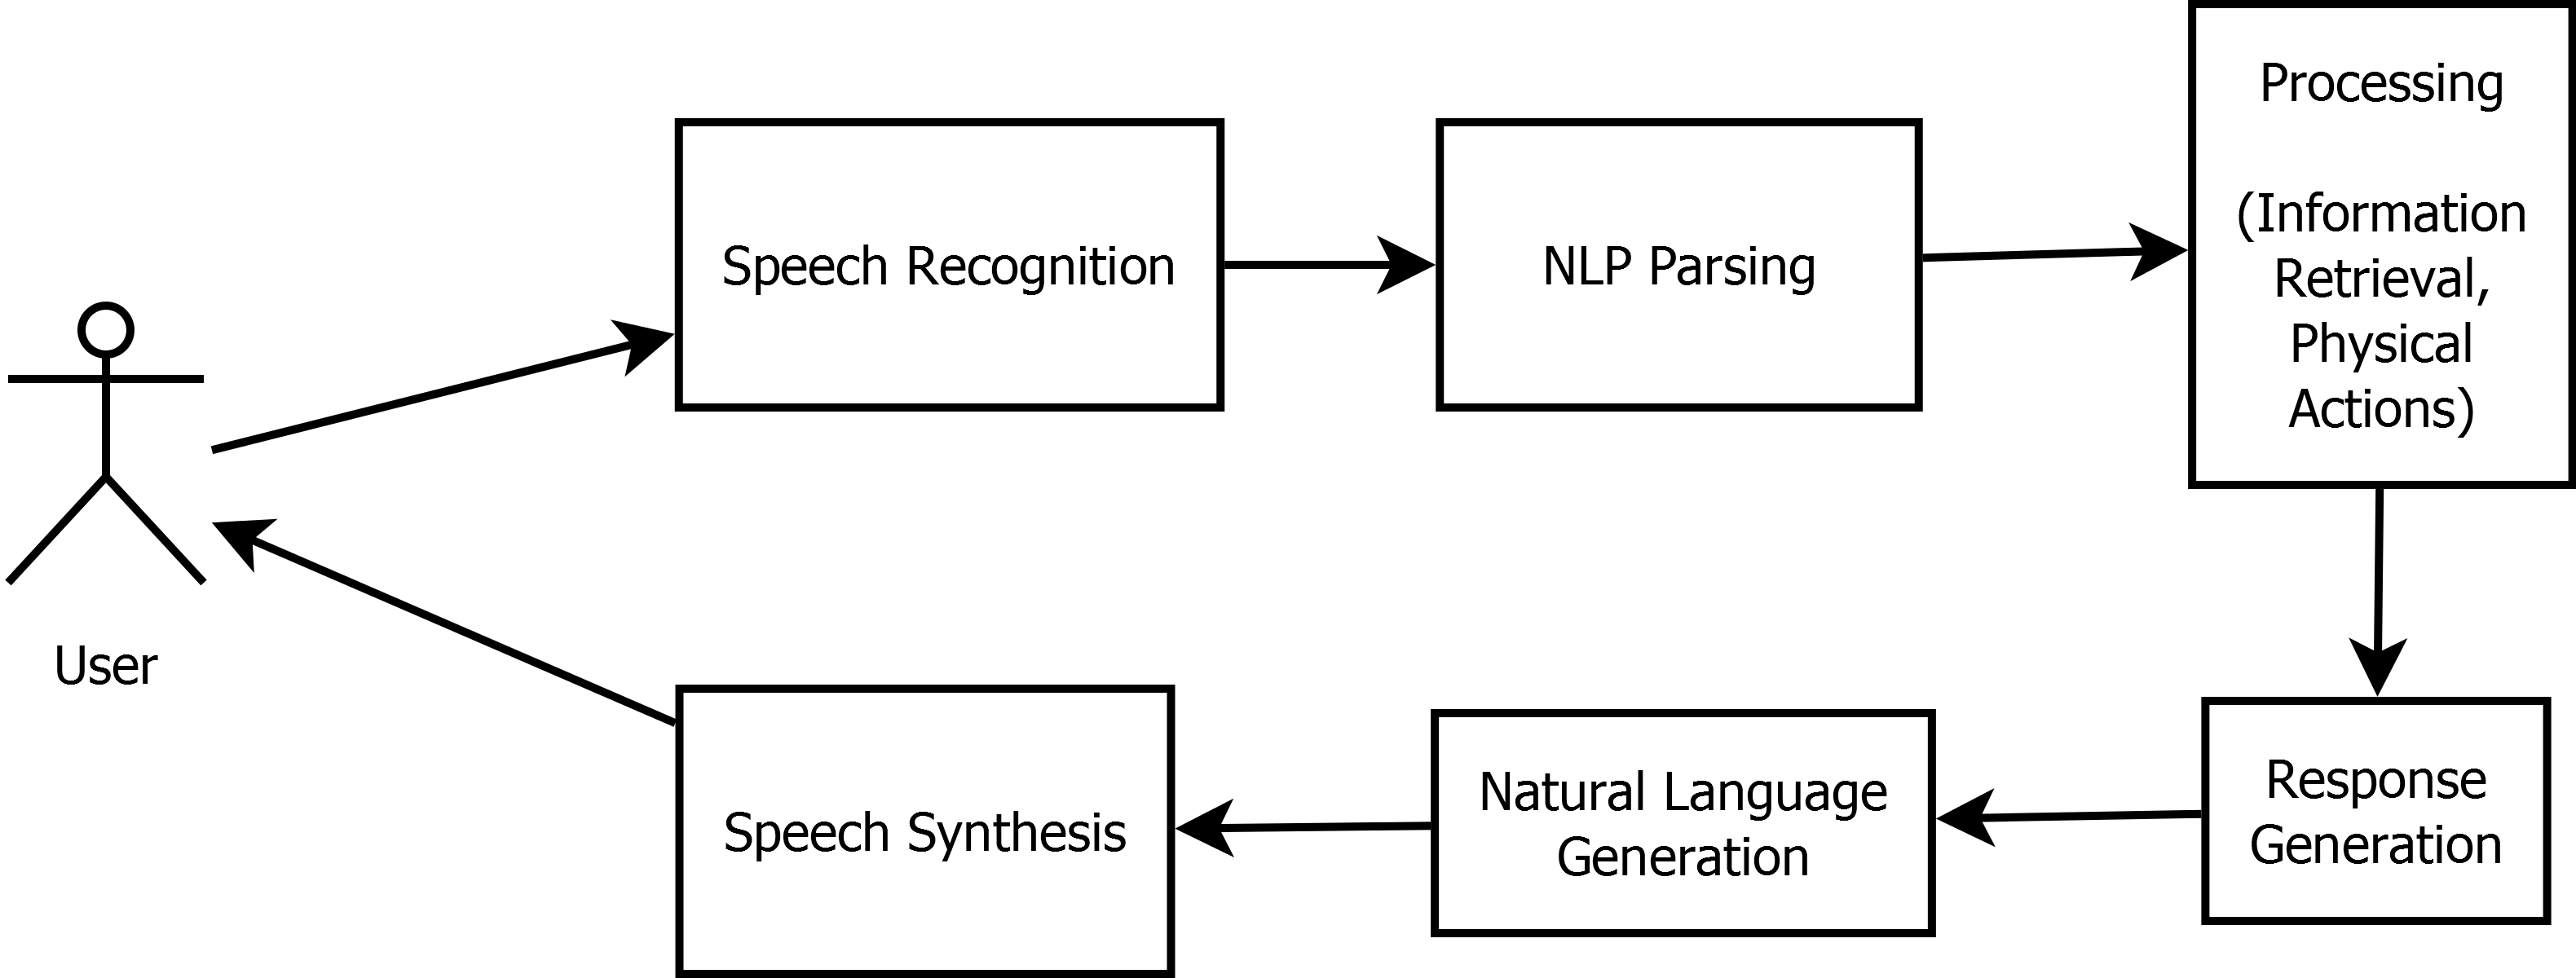
\includegraphics[width=0.8 \linewidth]{nlp-block.png}
\caption{A diagram showing the flow of information through a normal interaction
with a user in a generalized NLP system}
\label{nlp-block}
\end{figure}

In this thesis, we consider the following restricted NLG problem: given a
grammar, lexicon, and a communicative goal, output a valid English
sentence that satisfies this goal.  We call this problem "restricted", because
it assumes a level of knowledge about the context in which the generation
will occur.  In principle, the most general NLG problem is to produce a valid
sentence in an arbitrary language, using the entire grammar and lexicon available
in that language, to satisfy an arbitrary communicative goal.  In practice, we
rarely require this level of generality; it would be unnecessary for the concierge
program described above to be intimately familiar with the finer points of Klingon grammar.
In practice, therefore, our restricted problem is a reasonable one.

Previous work on this problem has taken two broad approaches.  On one hand we have
the classical planning approaches, which treat the problem of NLG as an AI planning
problem.  These systems have the advantage of being capable of finding acceptable
output in all circumstances where a perfect answer exists, but the disadvantage of
being unable to handle a probabilistic grammar in a structured way.  They also struggle
with completing a subset of the communicative goals, when full completion is not
possible.  On the other hand, there are statistical planners which work by examining the
most probable combinations of words and determining if any of those match the
meaning they are attempting to generate.  These have the advantage of completing
execution very quickly, and of taking advantage of Zipf's Law, which states broadly that
a very small subset of a language is used a very large proportion of the time.  They
have the disadvantage of requiring an inordinate amount of memory to be able to search
for the less-likely phrases and sentences which will occasionally need to be generated.
They also scale poorly with large grammar sizes.

We propose an algorithm which unifies these two approaches, and has, to some extent,
the advantages of both.  This algorithm gives
us the ability to efficiently search a large space (all possible natural language outputs) for 
one of many valid outputs.  We support probability in a structured way and allow
for generation using a large grammar.  We support partial completion of the communicative
goal, but strive for full completion when it is possible.  We allow for generation to stop
at any time and will return a partially-complete result very quickly.

We do this, broadly, by using probabilistic planning rather than classical planning.
Our algorithm is based in Monte-Carlo Tree Search, an increasingly
popular method for probabilistic planning.

We believe that if this algorithm were developed further, it could be useful as the
final step of a dialog system, or useful in generation situations where flexibility of the
generation system is crucial.  At present, it is already useful as the output stage of
a simple dialog system.  An efficient implementation would be able to take advantage
of multiprocessing and therefore run very well on a massively multiprocessing system,
enhancing performance substantially.

In chapter 2, we provide background information on NLG and probabilistic planning.  In chapter 3,
we discuss related work, including historical natural language generation frameworks.  We also
discuss the closest related system to ours, called CRISP.  In chapter 4, we present our framework
for natural language generation.  In chapter 5, we present our experimental evaluation of
our implementation, which shows that it performs comparably to the current state-of-the-art in
the field.  In chapter 6, we conclude by describing the potential applications and future work
using this method of generation.
\section{Related Work}
\include{ch2_relwork}
\section{Framework}
\include{ch3_framework}
\section{Experiments}
\include{ch4_experiment}
\section{Conclusion}
\include{ch5_conclusion}

% appendix
%\begin{appendices}               % Start of the Appendix Chapters.  If there is only
                                 % one Appendix Chapter, then use \begin{appendix}
%\include{app1_variables}
%\include{app2_workspace}
%\include{app3_r2}
%\include{code}                   % Including computer code listings
%\include{bibref}                 % a BibTeX reference
%\include{math}                   % Complex Equations from the UW Math Department
%\include{acro}                   % A discussion on generating PDF files.
%\end{appendices}                 % End of the Appendix Chapters.  ibid on \end{appendix}

%\bibliography{refs}              % Make the bibliography

%\include{vita}                  % Optional Vita, use \begin{vita} vita text \end{vita}
\end{document}

